\documentclass[12pt,openany,a4paper]{book}
\usepackage{graphicx}	% if you want encapsulated PS figures.

\usepackage{url} % more nicely formatted urls in the references
\usepackage[style=ieee]{biblatex}
\addbibresource{mybib.bib}
\renewcommand{\bibname}{References}

\usepackage{listings} % for pretty printing code

% If you use a macro file called macros.tex :
% \input{macros}
% Note: The present document has its macros built in.

% Number subsections but not subsubsections:
\setcounter{secnumdepth}{2}
% Show subsections but not subsubsections in table of contents:
\setcounter{tocdepth}{2}

\pagestyle{headings}		% Chapter on left page, Section on right.
\raggedbottom

\setlength{\topmargin}		{-5mm}  %  25-5 = 20mm
\setlength{\oddsidemargin}	{+10mm}  % rhs page inner margin = 25+10mm
\setlength{\evensidemargin}	{0mm}   % lhs page outer margin = 25mm
\setlength{\textwidth}		{150mm} % 35 + 150 + 25 = 210mm
\setlength{\textheight}		{240mm} % 

\renewcommand{\baselinestretch}{1.2}	% Looks like 1.5 spacing.

% Stop figure/tables smaller than 3/4 page from appearing alone on a page:
\renewcommand{\textfraction}{0.25}
\renewcommand{\topfraction}{0.75}
\renewcommand{\bottomfraction}{0.75}
\renewcommand{\floatpagefraction}{0.75}

% THEOREM-LIKE ENVIRONMENTS:
\newtheorem{defn}	{Definition}	% cf. \dfn for cross-referencing
\newtheorem{theorem}	{Theorem}	% cf. \thrm for cross-referencing
\newtheorem{lemma}	{Lemma}		% cf. \lem for cross-referencing

% HELPS CROSS-REFERENCING (All take a label as argument):
\newcommand{\eref}[1] {(\ref{#1})}		% (...)
\newcommand{\eq}[1]   {Eq.\,(\ref{#1})}		% Eq.~(...)
\newcommand{\eqs}[2]  {Eqs.~(\ref{#1}) and~(\ref{#2})}
\newcommand{\dfn}[1]  {Definition~\ref{#1}}	% Definition~...
\newcommand{\thrm}[1] {Theorem~\ref{#1}}	% Theorem~...
\newcommand{\lem}[1]  {Lemma~\ref{#1}}		% Lemma~...
\newcommand{\fig}[1]  {Fig.\,\ref{#1}}		% Fig.~...
\newcommand{\tab}[1]  {Table~\ref{#1}}		% Table~...
\newcommand{\chap}[1] {Chapter~\ref{#1}}	% Chapter~...
\newcommand{\secn}[1] {Section~\ref{#1}}	% Section~...
\newcommand{\ssec}[1] {Subsection~\ref{#1}}	% Subsection~...

% HELPS FORMATTING:
\newcommand{\teq}[1]	{\mbox{$#1$}}	% in-Text EQuation (unbreakable)
\newcommand{\qed}	{\hspace*{\fill}$\bullet$}	% end of proof

% MATHEMATICAL TEMPLATES:
% Text or math mode:
\newcommand{\half}	{\ensuremath{\frac{1}{2}}}	% one-half
\newcommand{\halftxt}	{\mbox{$\frac{1}{2}$}}	  	% one-half, small
% Math mode only:
% N.B. Parentheses are ROUND; brackets are SQUARE!
\newcommand{\oneon}[1]	{\frac{1}{#1}}		  % reciprocal
\newcommand{\pow}[2]	{\left({#1}\right)^{#2}}  % Parenthesized pOWer
\newcommand{\bow}[2]	{\left[{#1}\right]^{#2}}  % Bracketed pOWer
\newcommand{\evalat}[2]	{\left.{#1}\right|_{#2}}  % EVALuated AT with bar
\newcommand{\bevalat}[2]{\left[{#1}\right]_{#2}}  % Bracketed EVALuated AT
% Total derivatives:
\newcommand{\sdd}[2]	{\frac{d{#1}}{d{#2}}}		    % Short
\newcommand{\sqdd}[2]	{\frac{d^2{#1}}{d{#2}^2}}	    % 2nd ("SQuared")
\newcommand{\ldd}[2]	{\frac{d}{d{#1}}\left({#2}\right)}  % Long paren'ed
\newcommand{\bdd}[2]	{\frac{d}{d{#2}}\left[{#2}\right]}  % long Bracketed
% Partial derivatives (same sequence as for total derivatives):
\newcommand{\sdada}[2]	{\frac{\partial {#1}}{\partial {#2}}}
\newcommand{\sqdada}[2]	{\frac{\partial ^{2}{#1}}{\partial {#2}^{2}}}
\newcommand{\ldada}[2]	{\frac{\partial}{\partial {#1}}\left({#2}\right)}
\newcommand{\bdada}[2]	{\frac{\partial}{\partial {#1}}\left[{#2}\right]}
\newcommand{\da}	{\partial}

% ORDINAL NUMBERS:
\newcommand{\ith}	{\ensuremath{i^{\rm th}}}
\newcommand{\jth}	{\ensuremath{j^{\rm th}}}
\newcommand{\kth}	{\ensuremath{k^{\rm th}}}
\newcommand{\lth}	{\ensuremath{l^{\rm th}}}
\newcommand{\mth}	{\ensuremath{m^{\rm th}}}
\newcommand{\nth}	{\ensuremath{n^{\rm th}}}

% SINUSOIDAL TIME AND SPACE-DEPENDENCY FACTORS:
\newcommand{\ejot}	{\ensuremath{e^{j\omega t}}}
\newcommand{\emjot}	{\ensuremath{e^{-j\omega t}}}

% UNITS (TEXT OR MATH MODE, WITH LEADING PADDING SPACE IF APPLICABLE):
% NB: These have not been tested since being modified for LaTeX2e.
\newcommand{\pack}	{\hspace{-0.08em}}
\newcommand{\Pack}	{\hspace{-0.12em}}
\newcommand{\mA}	{\ensuremath{\rm\,m\pack A}}
\newcommand{\dB}	{\ensuremath{\rm\,d\pack B}}
\newcommand{\dBm}	{\ensuremath{\rm\,d\pack B\pack m}}
\newcommand{\dBW}	{\ensuremath{\rm\,d\pack B\Pack W}}
\newcommand{\uF}	{\ensuremath{\rm\,\mu\pack F}}
\newcommand{\pF}	{\ensuremath{\rm\,p\pack F}}
\newcommand{\nF}	{\ensuremath{\rm\,n\pack F}}
\newcommand{\uH}	{\ensuremath{\rm\,\mu\pack H}}
\newcommand{\mH}	{\ensuremath{\rm\,m\pack H}}
\newcommand{\Hz}	{\ensuremath{\rm\,H\pack z}}
\newcommand{\kHz}	{\ensuremath{\rm\,k\pack H\pack z}}
\newcommand{\MHz}	{\ensuremath{\rm\,M\pack H\pack z}}
\newcommand{\GHz}	{\ensuremath{\rm\,G\pack H\pack z}}
\newcommand{\J}		{\ensuremath{\rm\,J}}
\newcommand{\kg}	{\ensuremath{\rm\,k\pack g}}
\newcommand{\K}		{\ensuremath{\rm\,K}}
\newcommand{\m}		{\ensuremath{\rm\,m}}
\newcommand{\cm}	{\ensuremath{\rm\,cm}}
\newcommand{\km}	{\ensuremath{\rm\,k\pack m}}
\newcommand{\mm}	{\ensuremath{\rm\,m\pack m}}
\newcommand{\nm}	{\ensuremath{\rm\,n\pack m}}
\newcommand{\um}	{\ensuremath{\rm\,\mu m}}
\newcommand{\Np}	{\ensuremath{\rm\,N\pack p}}
\newcommand{\s}		{\ensuremath{\rm\,s}}
\newcommand{\ms}	{\ensuremath{\rm\,m\pack s}}
\newcommand{\us}	{\ensuremath{\rm\,\mu s}}
\newcommand{\V}		{\ensuremath{\rm\,V}}
\newcommand{\mV}	{\ensuremath{\rm\,m\Pack V}}
\newcommand{\W}		{\ensuremath{\rm\,W}}
\newcommand{\mW}	{\ensuremath{\rm\,m\Pack W}}
\newcommand{\ohm}	{\ensuremath{\rm\,\Omega}}
\newcommand{\kohm}	{\ensuremath{\rm\,k\Omega}}
\newcommand{\Mohm}	{\ensuremath{\rm\,M\Omega}}
\newcommand{\degs}	{\ensuremath{\rm^{\circ}}}

% LaTeX run-time type-in command:
%
% \typein{Enter \protect\includeonly{...} command (or just type RETURN):}
%
% Uncommenting this command makes LaTeX prompt you for the \includeonly
% list.  At the prompt
%
%	\@typein=
%
% you type
%
%	\includeonly{chap1,chap2}
%
% to include the files chap1.tex and chap2.tex and omit any others.
% To include every \include file, just hit RETURN.
% If you are running LaTeX from xtexsh, you may need to click the mouse
% in the LaTeX window to position the cursor at the \@typein prompt.








\begin{document}

\frontmatter
% By default, frontmatter has Roman page-numbering (i,ii,...).

\begin{titlepage}
\renewcommand{\baselinestretch}{1.0}
\begin{center}
\begin{figure}[h]

\includegraphics[width=\textwidth]{uq_logo.png}
\end{figure}
\vspace*{25mm}
\Huge\bf
		An Exploration of the Libra Testnet\\
\vspace{20mm}
\large\sl
		by\\
		CAMERON JAMES HARDER-HUTTON
		\medskip\\
\rm
		School of Information Technology and Electrical Engineering,\\
		The University of Queensland.\\
\vspace{30mm}
		Submitted for the degree of\\
		Bachelor of Engineering (Honours)
		\smallskip\\
\normalsize
		in the division of Software Engineering
		\medskip\\
\large
		22nd June, 2020		
\end{center}
\end{titlepage}

\cleardoublepage

\begin{flushright}
    Cameron Harder-Hutton\\
	23 Moriah St\\
	Boondall, QLD 4034\\
	Tel.\ 0400 879 112\\
	\medskip
	\today
\end{flushright}
\begin{flushleft}
    Prof Amin Abbosh\\
    Head of School (Acting)\\
    School of Information Technology and Electrical Engineering\\
    The University of Queensland\\
    St Lucia, QLD 4072\\
    \bigskip\bigskip
    Dear Professor Abbosh,
\end{flushleft}

In accordance with the requirements of the degree of Bachelor of
Engineering (Honours) in the division of 
Software Engineering, I present the
following thesis entitled ``An Explorationg of the Libra Testnet''.
This work was performed under the supervision of
Dr Marius Portmann.

I declare that the work submitted in this thesis is my own, except as
acknowledged in the text and footnotes, and has not been previously
submitted for a degree at The University of Queensland or any other
institution.

\begin{flushright}
	Yours sincerely,\\
	\medskip
    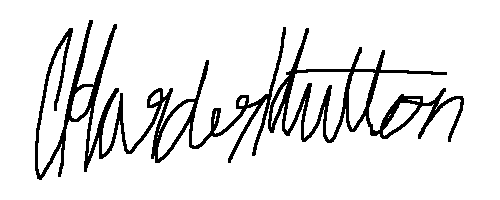
\includegraphics[width=0.25\textwidth]{imgs/signature.png} \\
	\medskip
	CAMERON HARDER-HUTTON.
\end{flushright}

\cleardoublepage

\chapter{Acknowledgments}

I would like to acknowledge my supervisor Dr Marius Portmann, for his help 
and guidance on undertaking this project. I would also like to thank him for 
offering this project in the first place, allowing me to do my thesis around a subject 
I am genuinely passionate about - blockchain. 

I would also like to acknowledge the (originally many, now few) developers working
on open source projects related to Libra. I am excited for the code from this 
project - and for myself - to become a part of that group.

\cleardoublepage

\chapter{Abstract}

Libra is a blockchain-based payments platform created and backed by Facebook
and their subsidiary company, Novi. On 
June 18, 2019 the Libra testnet was launched, allowing developers to interact with
the platform. This thesis is an exploration of such testnet. It investigates the data
which is available to be queried on the testnet and what can be learnt from it.
The way in which the testnet has changed over the first 12 months of its development is 
also explored.

Libra uses a leader-based Byzantine Fault-Tolerant consensus protocol. The role of the 
leader in leader-based consensus protocols is to receive votes from other nodes in 
the network, and propagate messages detailing the success/failure of the voting for that round.
Despite claiming to be random, the main contribution of this thesis is the discovery 
that Libra uses a reputation based algorithm for the selection of a round leader in 
consensus. Validator nodes - the name given to those whose computers
participate in the consensus - were less frequently chosen as round leader 
when they had a greater latency of communication with the rest of the network,
causing their votes to be counted less often.

\tableofcontents

\listoffigures
\addcontentsline{toc}{chapter}{List of Figures}

\listoftables
\addcontentsline{toc}{chapter}{List of Tables}

\cleardoublepage










\mainmatter

\chapter{Introduction}
\section{Project Significance}
In 2020, it is hard to see a future in which blockchain technology does not disrupt several industries.
In 2019, Venezuelans were able to use Bitcoin and Litecoin as a hedge against hyperinflation 
as a result of government corruption \cite{venezuela_btc, venezuela_btc2}. 
Louis Vuitton are able to use blockchain to help customers verify the authenticity of their designer goods \cite{blockchain_LV}.
And, healthcare institutions are using blockchain for contact tracing and secure 
medical records \cite{blockchain_healthcare, blockchain_healthcare2}.

Blockchain, however, is still very far from widespread consumer adoption as a 
trustworthy and reliable technology \cite{prewett_2020}. This is where the advent of Libra makes the space interesting.

Libra was announced on 18 June, 2019, as a new cryptocurrency being developed by Facebook \cite{isaac_popper_2019}.
Libra intends to be a global payment system, and to bring banking to the unbanked 
populations of the world \cite{libra_vision}. 
Unlike many cryptocurrencies, it intends to be a stable currency \cite{libra_whitepaper}.
Since April 2020, this definition has expanded to Libra becoming a global payment platform - incorporating many 
stable cryptocurrencies.
This project is a significant validation of blockchain technology to the greater public, and it
will be even more significant once it is officially released.

Many people have criticised Libra, stating that it is not a true cryptocurrency, needs regulation \cite{rirsh_tomanek} or that 
it poses a threat to the very nature of global finance \cite{petrou_20}. 
There is however, one absolute truth: Facebook has over 2.5 billion monthly active users \cite{facebook_stats}, so
regardless of whether you believe Libra is an abhorrent
misrepresentation of Satoshi's vision or not, if it can find its legs, it \textit{will} 
show consumers that there 
are faster, easier and cheaper ways to send money than using a bank \cite{taskinsoy}.

\section{Project Scope}
The project proposal entailed two parts: 
\begin{enumerate}
    \item The development of a 'blockchain explorer' for the Libra testnet, similar to those made 
    for other blockchains \cite{etherscan, blockchain_dotcom}, and
    \item The development of a custom Libra Node, within a local Libra testnet. This would facilitate 
    running simulations, threshold and stress testing, and observe network commmunication at a low level.
\end{enumerate}

However, as the project proceeded, the second goal was dropped in favour of 
a more thorough investigation of the first. There were two reasons for this:
\begin{enumerate}
    \item The endpoints through which information could be gathered from the Libra testnet 
    received breaking changes too frequently, each time requiring effort to update 
    data collection methods.
    \item Interesting information regarding validator voting and round leadership 
    was found which warranted further investigation.
\end{enumerate}

As such, the scope of this project is to be able to query and collect data from the Libra testnet.
It is the responsibility of technically capable individuals to conduct due 
dilligence of platforms such as Libra, since they are likely to affect the daily lives 
of many people in the not too distant future. With this in mind, the further goal of this 
project is to improve the security and user experience of Libra's end users, by 
keeping the blockchain accountable for the promises it makes.


\section{Outline}

Chapter \ref{__libra_blockchain} contains a detailed, technical explanation of the Libra blockchain:
Section \ref{__libra_blockchain:kc} details Key Concepts, section \ref{consensus_protocol} 
explains the Consensus protocol and section \ref{__lb:testnet} describesthe state of the testnet. 

Chapter \ref{__related_works} explores related works, with section \ref{__related_works:other_blockchains} 
detailing similar work done on other blockchains and section \ref{__related_works:libra} 
looking at other works done on the Libra testnet.

Chapter \ref{__data_collection} details the methodology followed in this project.
Section \ref{query_testnet_ledger} describes how data was collected, 
section \ref{local_data_storage} describes how data was stored and 
section \ref{web_app} describes the assoicated web application.

Chapter \ref{result_disc} presents the data and findings.
Section \ref{results:tx_data} presents data related to transactions,
section \ref{results:validator_voting_data} presents data related validator 
voting patterns and round leadership selection.
Section \ref{discussion} discusses the implications of these findings, as 
well as a way for the Libra developers to address the found concerns.

Chapter \ref{conc} conludes this thesis.
Section \ref{conc:summ} summarises the findings and 
section \ref{conc:future} describes future work.



\chapter{The Libra Blockchain}
\label{__libra_blockchain}
On June 18 2019, Facebook announced 'Libra' \cite{isaac_popper_2019}.
At this time, the project was just intended to be a digital currency and payment platform. Libra was branded as 
being a global, stable cryptocurrency - called Libra Coin - to facilitate the unbanked population of 
the world. \cite{libra_path_forward} Since then, Libra has pivoted goals. Libra 
is now a payments platform for the aforementioned Libra Coin, and global currency
stablecoins. Libra Coin itself is intended to be a stablecoin 
backed by the Libra Reserve - a basket of cash, cash equivalents and short-term 
government securities \cite{libra_whitepaper}.

Libra is a permissioned blockchain, meaning that appoval must be given by a governing
body in order to participate in validating transactions on the Libra network. 
Such governing body is called the Libra Association, an independent 
membership organisation in Geneva, Switzerland - of which Facebook remains 
a member. The original white paper 
intended for Libra to transition to a permissionless blockchain 
- like Bitcoin and Ethereum - in five years. However, the April 2020 revision of the 
Libra white paper has removed this intention, citing regulatory dissatisfaction 
\cite{libra_whitepaper, verge_libra_shift}.
According to documents released by the Libra Association \cite{libra_association_member}, an organisation must
meet the folowing criteria to become a member:
\begin{itemize}
    \item Be able to run either a self-hosted or cloud-hosted Validator Node,
    \item Market value greater than \$1 billion USD \textit{or} Customer balances greater tha \$500 million USD,
    \item Reach more than 20 million people a year in more than one country,
    \item Be recognised as a top-100 industry leader.
\end{itemize}

\section{Key Concepts}
\label{__libra_blockchain:kc}
\subsection{Nodes}
\textit{Validator Node} is the term given to a full Libra node which participates 
in consensus \cite{libra_smr}. At launch, Libra intends to have 100 validator nodes from a diverse selection of 
organisations and geographic locations \cite{libra_path_forward, libra_whitepaper}.

\begin{figure}[h]
    \caption{\sl The components of a Libra Validator Node \cite{libra_validator_node}}
    \label{validator_node_img}
    \begin{center}
    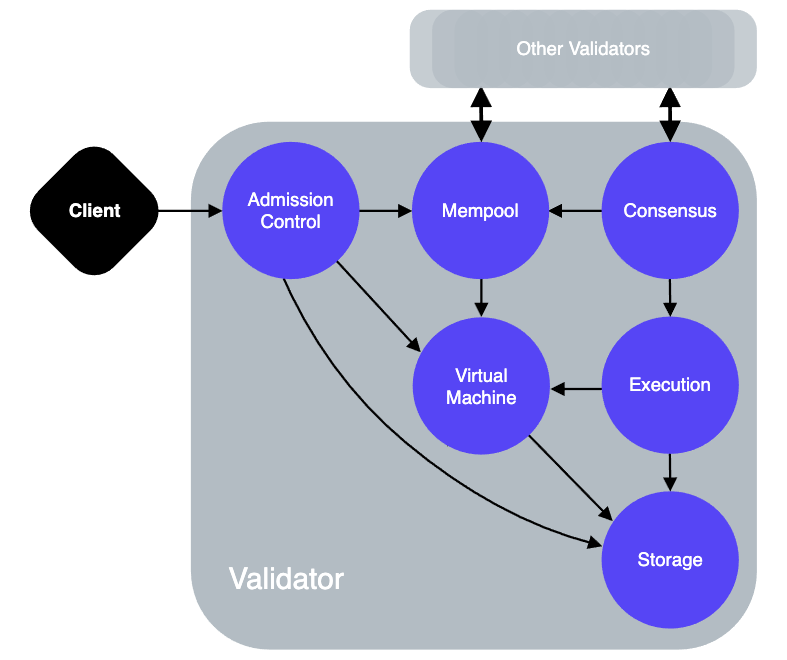
\includegraphics[width=0.7\textwidth]{imgs/validator_node.png}
    \end{center}
\end{figure}

The six components in Figure \ref{validator_node_img} serve the following purposes:
\begin{itemize}
    \item \textbf{Admission Control:} External interface for client queries. 
    Newly submitted transactions and queries about the state of the ledger or an account are received here,
    \item \textbf{Mempool:} Contains transactions awaiting execution, updates to this component are
    share amongst validators,
    \item \textbf{Consensus:} The component responsible for executing the consensus protocol,
    see \ref{consensus_protocol},
    \item \textbf{Virtual Machine:} Responsible for speculatively executing the transaction scripts to validate them see \ref{kc_move}
    \item \textbf{Execution:} Responsible for executing transactions committed to the blockchain,
    \item \textbf{Storage:} The ledger itself, see \ref{kc_ledger}.
\end{itemize}

There are two other types of participants in the Libra network: \textit{Full nodes} and \textit{Clients}.

\textit{Full nodes} fulfil a role similar to the Admission Control component of a validator node, 
by answering ledger queries from clients. Full nodes also keep local storage of the 
ledger \cite{libra_full_nodes}. At present, it is not possible to run a full node 
connected to the official Libra testnet.

\textit{Clients} refers to any computer or wallet submitting transactions or querying the ledger state
\cite{libra_full_nodes}. 

\subsection{Accounts \& Wallets}
The term account and wallets are used interchangeably in Libra. Accounts are 
simply an address with which some Move Resources (see \ref{kc_move}) are 
associated \cite{libra_validator_node, libra_technical_paper}.

\subsection{Ledger}
\label{kc_ledger}
The underlying data storage method of Validator and Full nodes in the Libra 
network is a RocksDB database \cite{libra_storage}. A RocksDB instance 
contains a versioned database of transactions. Each version is a 
single transaction, identified by a monotonically 
increasing unsigned 64-bit integer starting from the Genesis: version 0 
\cite{libra_validator_node, libra_technical_paper, libra_smr}. Versions 
are stored in a Merkle Tree, with each version existing as its own leaf node
\cite{libra_technical_paper}.

\subsection{Move Language}
\label{kc_move}
Move is the programming language in which Libra transactions and (eventually) 
smart contracts are written. Move is an executable bytecode langauge - meaning that it 
is very fast and efficient to transport, store, and validate.
\textit{Types} in Move are called Resources. Resources cannot be copied, only moved 
in memory. Only the Libra Association is able to create or destory Move Resources \cite{libra_move}.

\section{Consensus Protocol}
\label{consensus_protocol}
Libra implements a leader-based Byzantine Fault Tolerant (BFT) consensus protocol called LibraBFT \cite{libra_technical_paper}.
LibraBFT is covered in detail by an article authored by the Libra Association 
entitled "State Machine Replication in the Libra Blockchain" \cite{libra_smr}. 
The following is a high level summary of that article.
Voting is organised into \textit{rounds} and each round has a \underline{randomly chosen}
leader. The leader is sometimes referred to at the \textit{block proposer}, as the leader 
proposes a block of transactions, and validators vote if that block is valid.
Once \textit{2f + 1} votes are received, the block is certified.

When a leader proposes a new block, it must extend from a certified block, or 
a WriteSet Transaction. A certified block \textit{k} is not committed to the ledger until 
a 3-chain of blocks extending from \textit{k} is certified. This is better illustrated in
Figure \ref{3_chain}.

\begin{figure}[h]
    \caption{\sl Proposed blocks and consensus rounds \cite{libra_smr}}
    \label{3_chain}
    \begin{center}
    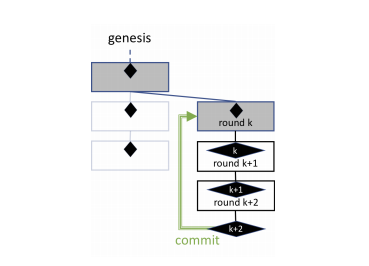
\includegraphics[width=0.7\textwidth]{imgs/3_chain.png}
    \end{center}
\end{figure}


\section{Testnet}
\label{__lb:testnet}
The Libra testnet allows for creating addresses, minting Libra coins (LBR) 
and making peer to peer transactions. It is also possible to deploy a local version 
of the Libra network.

Transactions committed to the ledger can be queried by version, or by association with a 
particular address. Unfortunately, that is the only information available.
Since Libra is a permissioned blockchain, it is not possible to connect directly 
to the validator nodes, only through the specified API endpoints (section \ref{json_api}).
So, data on how validator nodes communicate and propagate messages cannot be recorded.

\subsection{Transaction Types}
The types of transactions currently being used in the Libra testnet can be seen
in \cite{libra_jsonrpc_spec}. there are four types:
\begin{itemize}
    \item \textbf{BlockMetadata Transactions:} These transactions contain metadata for each block.
    Its return fields are detailed in \ref{available_data},
    \item \textbf{WriteSet Transaction:} The genesis version or any updates to the validator set are WriteSet transactions.
    \item \textbf{User Transaction:} Any peer to peer or mint transactions. Its return fields are detailed in \ref{available_data},
    \item \textbf{Unknown Transaction:} A blanket type for transactions (for now) that execute custom, but still valid Move scripts.
\end{itemize}



\subsection{JSON-RPC API}
\label{json_api}
The methods and return types for the JSON-RPC API can be seen here \cite{libra_jsonrpc_spec}.

\subsection{Types of Available Data}
\label{available_data}
Fields from block metadata transaction that were used in the data collection of this project 
can be seen in Table \ref{bm_datatypes_table}. The raw version of this transaction is 
in Appendix \ref{appendix:json_txns:bm}.

\begin{table}[h!]
    \caption{\sl Relevant information returned from JSON-RPC call (Block Metadata transaction)}
    \label{bm_datatypes_table}
\begin{center}
\begin{tabular}{ |c|c| } 
    \hline
    Value & Type \\
    \hline
    Time Proposed & Unix Timestamp \\
    Proposer & 512 bit hex address \\
    Transaction Type & String \\
    Time Committed & Unix Timestamp \\
    Transaction Version & Int \\
    VM Status & Int \\
    \hline
\end{tabular}
\end{center}
\end{table}

Fields from user transactions that were used in the data collection of this project 
can be seen in Table \ref{tx_datatypes_table}. The raw version of this transaction is 
in Appendix \ref{appendix:json_txns:p2p}.

\begin{table}[h!]
    \caption{\sl Relevant information returned from JSON-RPC call (User transaction)}
    \label{tx_datatypes_table}
\begin{center}
\begin{tabular}{ |c|c| } 
    \hline
    Value & Type \\
    \hline
    Time Proposed & Unix Timestamp \\
    Sender & 512 bit hex address \\
    Receiver & 512 bit hex address \\
    Amount & Int \\
    Gas Amount & Int \\
    Transaction Type & String \\
    Transaction Version & Int \\
    VM Status & Int \\
    \hline
\end{tabular}
\end{center}
\end{table}

\subsection{Previous Revisions}
The testnet originally used gRPC \cite{grpc} for transporting data to clients making 
queries on the testnet. gRPC is a remote procedure call framework developed by Google which allows for 
language-agnosting types to be defined (called protobufs) and built in the end
user's language of choice \cite{grpc_detail}. 
In May 2020, Libra decided to move towards JSON-RPC \cite{libra_jsonrpc}. This was done in 
order to make Libra more easily accessible to developers by using a remote procedure call 
framework more popular in the cryptocurrency community.

\chapter{Related Works}
\label{__related_works}
\section{Investigation into Other Blockchains}
\textit{The following sections (\ref{pp1}, \ref{pp2}, and \ref{pp3}) were taken 
and revised from the project proposal document \cite{project_proposal}.}
\label{__related_works:other_blockchains}
\subsection{Ethereum Crawler}
\label{pp1}
\cite{eth_crawler} implemented a network crawler on the Ethereum network. 
Ethereum is a permissionless blockchain which facilitates the development 
of decentralised applications (dApps) through the implementation of Smart 
Contracts \cite{vitalik}. The development of dApps is also an intended features of the 
Libra blockchain \cite{libra_path_forward}.

The crawler required the bootstrapping of a full Ethereum node, communicated 
between peers using RPC calls and queried physical memory of the local storage to 
obtain information from the blockchain. The data gathered was used to 
visualise a number of insights from the data. Transaction throughput over time 
was able to be visualised with timestamps on transactions, as well as during 
which times the most assets were being transferred. \cite{eth_crawler} also 
observed ‘zombie contracts’ - those with no executable code in the smart 
contract, usually because of an error on the part of the author - and found 
that they increased linearly over time, implying that education surrounding 
verifying the correctness of a contract before deployment did not improve over 
time. This is an interesting discovery, considering that the Move language 
specification document actually quotes the difficulty in writing verifiable 
Ethereum Smart Contracts \cite{libra_move}.

\cite{eth_crawler} was able to see the geographic dispersity of nodes on the 
Ethereum network, noting that most were centralised in western countries, 
Russia and China. Unfortunately, this required access to the IP addresses of 
nodes which isn’t intended to be possible in the Libra network since it is 
permissioned.


\subsection{Ripple Crawler}
\label{pp2}
\cite{ripple_crawler}
Another network crawler was developed for the Ripple network 
in \cite{ripple_crawler}. Ripple is another permissionless blockchain, 
however it was developed to be purely a payment platform. This crawler obtained 
information on transaction history via remote procedure calls to Ripple’s 
public APIs and gathered the transaction history of specific addresses using 
Ripple’s own tools for this. This information was used to build a list of all 
the wallets on the ledger and compute the links between 
them. \cite{ripple_crawler} was able to classify wallets as dormant/active 
based on their transaction history. 

\cite{ripple_crawler} employed a clustering of Ripple nodes into highly 
connected communities and determined, unsurprisingly, that the most highly 
connected communities were those near ‘gateway nodes’, nodes that deposit 
Ripple currency into wallets when users deposit fiat. A clustering of public 
wallets was also implemented to link groups of wallets that all belonged to the 
same individual. In regards to wallets, implementing similar advanced analysis 
of transaction history on the Libra blockchain would allow computation of more 
insightful statistics such as the number of active  or the number of unique 
addresses on the network.


\subsection{HyperLedger Fabric Crawler}
\label{pp3}

In \cite{hyperledger_analysis}, a network analysis was conducted on Hyperledger 
Fabric. Hyperledger is a Blockchain-as-a-Service (BaaS) platform which provides 
permissioned blockchain solutions for businesses 
[ref]. \cite{hyperledger_analysis} deployed a new, permissioned blockchain on 
the Hyperledger network and ran 10 nodes locally on two separate computers, 
varying the ‘workload’ (amount transactions submitted to the network). The goal 
of this project was to assess the claims of Hyperledger is relation to 
execution time, latency and throughput. The experiment was repeated with 20 
total nodes and higher workloads in order to assess the scalability of 
Hyperledger Fabric. The investigation verified that Hyperledger Fabric 
performed at its advertised levels and was consistent despite varying amounts 
of nodes and submitted transactions. 



\section{Explorers on the Libra Testnet}
\label{__related_works:libra}
There are three active explorers for the Libra Testnet: Librabrowser.io, MoveOnLibra and LibExplorer.

\subsection{LibraBrowser}
Librabrowser.io \cite{librabrowser} allows users 
to see recent transactions, search for transactions by address or version. For Block Metadata 
transactions Librabrowser.io displays on the version number. For User Transactions,
they display the version number, status, transaction type, sender, receiver, amount, expiration time,
sequence number, gas used, maximum gas amount, public key, signature and script hash.
The expose their own API, which allows developers to request information similar to that
which can be queried directly from the testnet. However, they only offer information on user transactions
and do not appear to store any data relating to block metadata transactions. 
Librabrowser.io does not display any statistics or analysis of the transactions 
on the blockchain.
The developers behind this site used to have a project for this explorer open sourced
and on GitHub but it has been removed.


\subsection{MoveOnLibra}
MoveOnLibra is the only open source development of a Libra explorer \cite{mol}. Similar to Librabrowser.io,
they do not display any statistics related to engagement on the Libra testnet, however, they do not 
store any of the data from the testnet - instead make queries in real time to serve 
user requests \cite{mol_explorer}. This also makes it the only real-time explorer.
MoveOnLibra also exposes their own API endpoints.
The code for the MoveOnLibra Explorer can be seen at \cite{mol_explorer}. Their 
ability to query the testnet is based on open source projects by GitHub user 
'yuan-yx' \cite{yuan_libra_client, yuan_libra_grpc}.



\subsection{LibExplorer}
LibExplorer \cite{libexplorer} has all the functionality of Librabrowser and 
MoveOnLibra, however it also displays some statistics relating to testnet engagement.
The following statistics can be seen on LibExplorer, related to the current testnet revision:
\begin{itemize}
    \item Latest version,
    \item Total number of transactions,
    \item Average number of transactions per second (TPS),
    \item Proportion of P2P to Mint transactions, 
    \item Total supply of minted Libra coins,
    \item Total number of unique addresses.
\end{itemize}
The following statistics can be seen on a 24 hour and 72 hour timeframe, however do
not appear to be functional as of the testnet's introduction of custom transaction types in May 2020:
\begin{itemize}
    \item Number of Transactions,
    \item Address growth,
    \item Libra coin supply,
    \item Transaction fees,
    \item Average gas fee,
    \item TPS.
\end{itemize}

\section{Literature on Libra}
Currently, there are no technical articles regarding Libra.
There are however, two papers which look at Libra from an economics 
perspective \cite{taskinsoy, rirsh_tomanek}.


\chapter{Data Collection Methodology}
\label{__data_collection}
Due to the nature of open source development and Libra being in its infancy, the 
methodology for data collection was constantly evolving.
Code conducting data collection often needed to be rewritten to work with the latest 
non-backwards compatible, breaking change. Further, data analysis and local storage 
needed to be rewritten to account for any changes to the data available. Information 
on how to deploy and run the code assoicated with this project can be seen in 
Appendix \ref{appendix:project_code}.

Over the course of the project, the evolution of gathering data from the Libra
Testnet went through five main phases:

\begin{enumerate}
    \item gRPC \& protobuf (June 2019 - September 2019),
    \item gRPC \& LCS (September 2019 - May 2020),
    \item The introuction of Block Metadata (December 2019),
    \item JSON-RPC and deprecation of gRPC (May 2020 - present),
    \item The introduction of custom transaction types (May 2020 - present).
\end{enumerate}

\section{Querying the Testnet Ledger}
\label{query_testnet_ledger}
Initially, the Libra testnet was only able to be queried via gRPC. This entailed downloading 
langauge-agnostic type definitions (called protobuf) for libra types from the Libra repository and 
building them in a language of choice. Python was used at this stage since its simplicitly
allowed for rapid development of code to work with the constantly changing project.

On 19 August, 2019, Libra announced they would be moving away from protobuf and using 
Libra Canonical Serialisation (LCS) for storing and serving client queries of the 
testnet \cite{libra_lcs}.

As mentioned previously, the gRPC API was deprecated on 11 June 2020 in favour of 
JSON-RPC \cite{libra_jsonrpc}. In order to be able to submit working code as a part 
of this project, a new interface with the Libra Testnet had to be written.

The JSON-RPC API proved to be much simpler to work with, allowing the batching of queries 
for up to 1 million transactions at a time to be returned directly in JSON. This 
removed the necessiy to convert binary into JSON types using LCS.

\section{Local Data Storage}
\label{local_data_storage}
The downloaded ledger data was converted into JSON for easy storage and use later.
Initially, local storage space was negligible since there were few transactions 
being executed on the testnet. Following the introduction of Block Metadata transactions, a new 
method had to be used as one day's worth of testnet data was approximately 600MB

At this point, a NoSQL database was chosen for the storage. This was decided because 
Libra itself uses a NoSQL database to store its ledger on disk - RocksDB \cite{libra_storage}.
RocksDB is an open source, key-value (NoSQL) database also developed and maintained by Facebook
\cite{rocksdb}. Further, NoSQL databases allow data to be organised in a less structured way,
which makes development easier when the data models are constantly changing \cite{nosql_2, nosql_advantages}.
Because of these two factors, it was decided that NoSQL was more appropriate that SQL for this 
project.

User transactions were still stored in persistent JSON on disk, as they number 
of these transactions was still few enough that the memory needed to store them 
was negligible. Block metadata transactions were not stored in memory, but were parsed to
extract the block proposer and previous block voters, update statistics in the 
database with this information and then discarded.

\section{Web Application}
\label{web_app}
A \textit{simple} web application was developed in React to display this 
information, and act as a proof-of-concept for real-time connectivity to the Libra
testnet. The application is able to query recently committed transactions in real time
and display statistics which are calculated and stored in the database.

\chapter{Results and Discussion}
\label{result_disc}
\section{Transaction Data}
\label{results:tx_data}
The data presented in this section is from 28 May 2020 to 18 June 2020. 
There were two resets of the testnet during this time, as such, the data comes 
from 3 testnet revisions.
\begin{itemize}
    \item Testnet Sample 1 (28/05/2020 - 02/06/2020) - which contains 27 million transactions,
    \item Testnet Sample 2 (03/06/2020 - 09/06/2020) - which contains 25 million transactions,
    \item Testnet Sample 3 (10/06/2020 - 18/06/2020) - which contains 35 million transactions.
\end{itemize}

\begin{table}[h!]
    \caption{\sl Transaction data from Testnet Sample 128/05/2020 - 02/06/2020}
    \label{tx_table_1}
\begin{center}
\begin{tabular}{ |c|c| } 
    \hline
    Total Volume LBR Minted & 1,821,961,010 \\
    \hline
    Total LBR Transaction Volume & 15,020,134,142 \\
    \hline
    Total Number Unique Addresses & 62 \\
    \hline
    Total Number User Transactions & 125 \\
    \hline
    Total Number P2P Transactions & 82 \\
    \hline
    Total Number Mint Transactions & 43 \\
    \hline
    Total Number Custom Transactions & 171 \\
    \hline
\end{tabular}
\end{center}
\end{table}

\begin{figure}[h!]
    \caption{\sl Address topology from Testnet Sample 1 28/05/2020 - 02/06/2020}
    \label{tx_topology_1}
    \begin{center}
    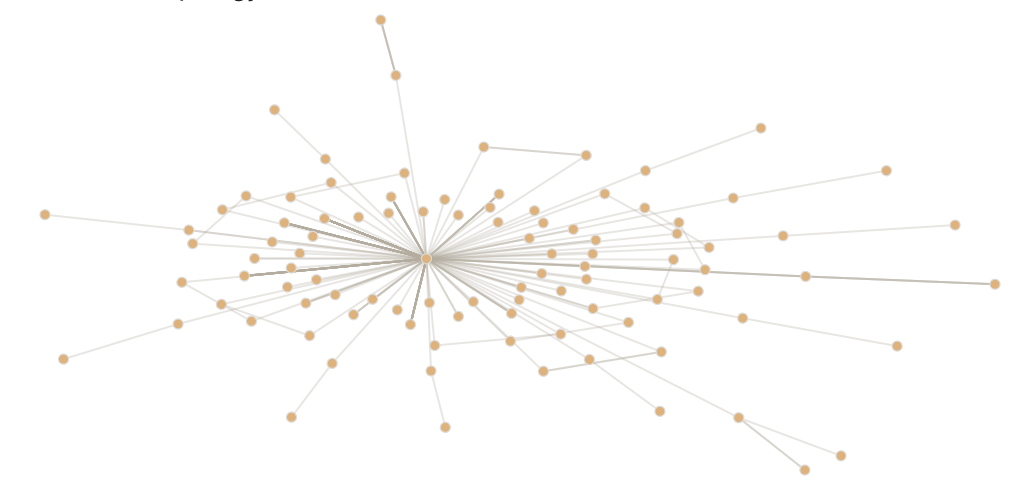
\includegraphics[width=0.7\textwidth]{imgs/tx_topology_2.png}
    \end{center}
\end{figure}

Figure \ref{tx_topology_1} shows the topology of addresses on the Libra network 
from this testnet revision (custom transactions removed). All coins on the network 
come from a single source, with very little peer to peer transactions being seen. 
Note: many addresses sent their LBR back to the minting address in this testnet, which
accounts for the still large number of P2P transactions.

\begin{table}[h!]
    \caption{\sl Transaction data from Testnet Sample 2 03/06/2020 - 09/06/2020}
    \label{tx_table_2}
\begin{center}
\begin{tabular}{ |c|c| } 
    \hline
    Total Volume LBR Minted & 949,202,440 \\
    \hline
    Total LBR Transaction Volume & 2,170,657,610 \\
    \hline
    Total Number Unique Addresses & 43 \\
    \hline
    Total Number User Transactions & 81 \\
    \hline
    Total Number P2P Transactions & 17 \\
    \hline
    Total Number Mint Transactions & 64 \\
    \hline
    Total Number Custom Transactions & 90 \\
    \hline
\end{tabular}
\end{center}
\end{table}

\begin{table}[h!]
    \caption{\sl Transaction data from Testnet Sample 3 10/06/2020 - 18/06/2020}
    \label{tx_table_3}
\begin{center}
\begin{tabular}{ |c|c| } 
    \hline
    Total Volume LBR Minted & 671,391,071 \\
    \hline
    Total LBR Transaction Volume & 15,020,134,142 \\
    \hline
    Total Number Unique Addresses & 159 \\
    \hline
    Total Number User Transactions & 190 \\
    \hline
    Total Number P2P Transactions & 57 \\
    \hline
    Total Number Mint Transactions & 133 \\
    \hline
    Total Number Custom Transactions & 322 \\
    \hline
\end{tabular}
\end{center}
\end{table}

\section{Voting Data}
\label{results:validator_voting_data}
There are three sets of data presented in this section. One from prior to the deprecation of 
the gRPC API and two from afterwards.

The first data set contain information about the number of times each validator 
was selected as a leader, and the number of votes that validator was able to cast.
The latter data sets only contain information about the number of times each validator was 
selected as leader, since the JSON-RPC API does not contain information about 
individual validator votes.

Note that the validator addresses have been shortened to their first four digits
for simplicity. The full addresses can be seen in Appendix \ref{appendix:val_addr_1}, 
\ref{appendix:val_addr_2} and \ref{appendix:val_addr_3}, respectively.

\subsection{Testnet Sample 1: 28/05/2020 - 02/06/2020}
The raw validator voting data from this version of the testnet can be seen in Table 
\ref{validator_table_1}. From Figure \ref{validator_pie_1}, it is apparent that all 
validators except \textit{65fe} were selected as round leader (block proposer) an 
approximately equal number of times. Further, Figure \ref{validator_votes_1} shows that
validator \textit{65fe} also had the fewest number of votes counted during consensus.

\begin{table}[h!]
    \caption{\sl Validator voting data from Testnet 28/05/2020 - 02/06/2020}
    \label{validator_table_1}
\begin{center}
\begin{tabular}{ |c|c|c| } 
    \hline
    Validator Address & Number of Blocks Proposed & Number of Votes Counted \\
    \hline
    \hline
    0e5c... & 4,659,743 & 26,406,710 \\
    \hline
    4c9e... & 4,725,392 & 26,561,253 \\
    \hline
    65fe... & 3,718,246 & 19,473,768 \\
    \hline
    b1aa... & 4,711,154 & 26,497,856 \\
    \hline
    dbd8... & 4,703,143 & 26,179,222 \\
    \hline
    fe5d... & 4,481,968 & 24,801,950 \\
    \hline
\end{tabular}
\end{center}
\end{table}

\begin{figure}[h]
    \caption{\sl Pie chart displaying block proposer proportions from Testnet 28/05/2020 - 02/06/2020}
    \label{validator_pie_1}
    \begin{center}
    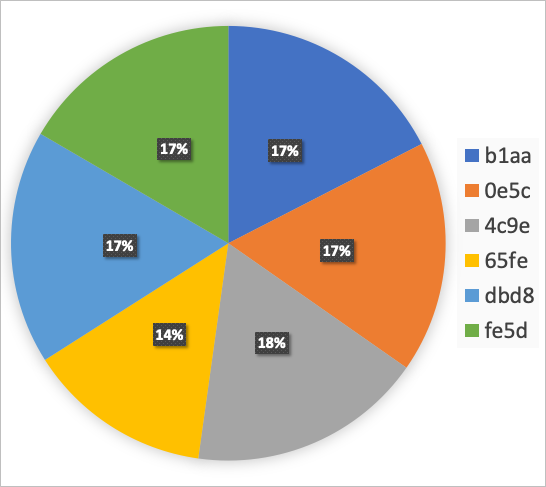
\includegraphics[width=0.7\textwidth]{imgs/testnet_validator_pie_1.png}
    \end{center}
\end{figure}

\begin{figure}[h]
    \caption{\sl Number of votes counted per validator from Testnet 28/05/2020 - 02/06/2020}
    \label{validator_votes_1}
    \begin{center}
    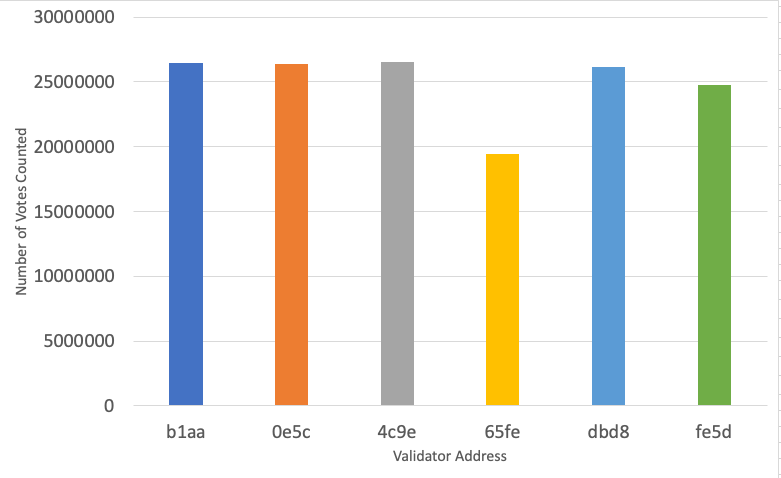
\includegraphics[width=0.7\textwidth]{imgs/testnet_validator_votes_1.png}
    \end{center}
\end{figure}

\subsection{Testnet Sample 2: 03/06/2020 - 09/06/2020}
The raw validator voting data from this version of the testnet can be seen in Table 
\ref{validator_table_2}. From Figure \ref{validator_pie_2}, it is apparent that all 
validators except \textit{987e} were selected as round leader (block proposer) an 
approximately equal number of times.
\begin{table}[h!]
    \caption{\sl Validator voting data from Testnet 03/06/2020 - 09/06/2020}
    \label{validator_table_2}
\begin{center}
\begin{tabular}{ |c|c| } 
    \hline
    Validator Address & Number of Blocks Proposed \\
    \hline
    \hline
    987e... & 2,690,592 \\
    \hline
    7bbc... & 4,267,926 \\
    \hline
    65fe... & 4,263,774 \\
    \hline
    b1aa... & 4,169,442 \\
    \hline
    2d4c... & 4,346,877 \\
    \hline
    4500... & 4,259,389 \\
    \hline
\end{tabular}
\end{center}
\end{table}

\begin{figure}[h]
    \caption{\sl Pie chart displaying block proposer proportions from Testnet 03/06/2020 - 09/06/2020}
    \label{validator_pie_2}
    \begin{center}
    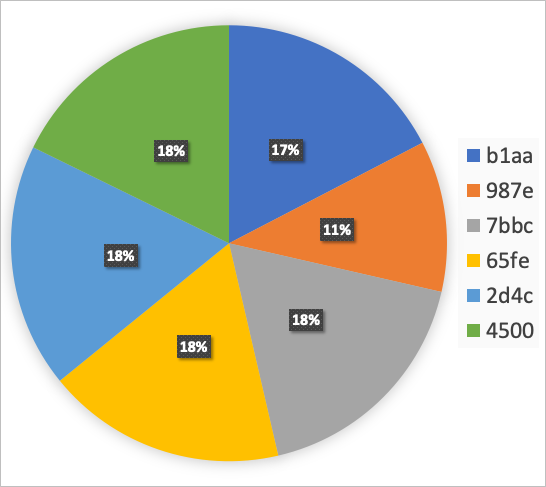
\includegraphics[width=0.7\textwidth]{imgs/testnet_validator_pie_2.png}
    \end{center}
\end{figure}

\subsection{Testnet Sample 3: 10/06/2020 - 18/06/2020}
The raw validator voting data from this version of the testnet can be seen in Table 
\ref{validator_table_3}. From Figure \ref{validator_pie_3}, it is apparent that all 
validators except \textit{65fe} were selected as round leader (block proposer) an 
approximately equal number of times.
\begin{table}[h!]
    \caption{\sl Validator voting data from Testnet 10/06/2020 - 18/06/2020}
    \label{validator_table_3}
\begin{center}
\begin{tabular}{ |c|c| } 
    \hline
    Validator Address & Number of Blocks Proposed \\
    \hline
    \hline
    987e... & 5,869,035 \\
    \hline
    7bbc... & 5,916,089 \\
    \hline
    65fe... & 5,097,108 \\
    \hline
    b1aa... & 5,987,350 \\
    \hline
    2d4c... & 6,076,875 \\
    \hline
    4500... & 6,053,543 \\
    \hline
\end{tabular}
\end{center}
\end{table}

\begin{figure}[h]
    \caption{\sl Pie chart displaying block proposer proportions from Testnet 10/06/2020 - 18/06/2020}
    \label{validator_pie_3}
    \begin{center}
    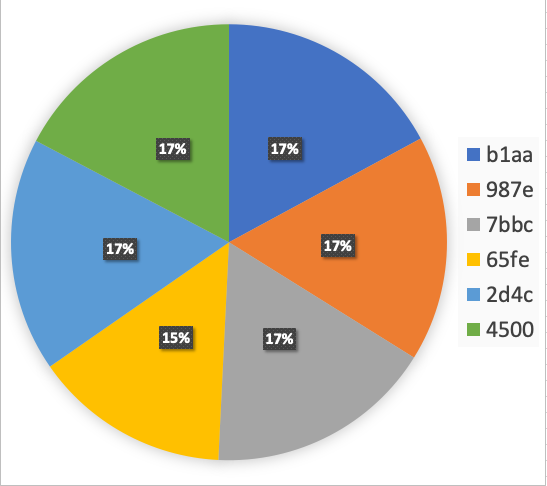
\includegraphics[width=0.7\textwidth]{imgs/testnet_validator_pie_3.png}
    \end{center}
\end{figure}

\section{Discussion}
\label{discussion}
There is little interesting information that can be taken from transaction data
on the testnet, since the data corresponds to pretend currency. Because of this,
the discussion around this data will focus on the validator data.

In every analysed revision of the testnet it is seen that one validator is nominated 
as block leader a significantly fewer amount of times than the rest. In order to understand why 
this is, let's explore the consensus protocol further.

Since LibraBFT is a Byztantine Fault-Tolerant protocol, \textit{2f + 1} validators 
- a \textit{greater than} two-thirds majority - must be recorded in order to certify a block.
When there are six validators, five votes must be recorded. Once the five votes are reached 
then the sixth is not needed. Assuming that all of the testnet validators are 
behaving honestly, then the validator whose vote is counted the least number of times 
is determined to be the \textit{least connected} to the rest of the network.

According to \cite{libra_technical_paper, libra_smr}, the time at which validators 
send messages is determined by the order in which they receive and parse other messages.
The time at which validators receive messages is determined by the time in which they are 
sent and the transmission latency between two validators. This would explain why 
in Testnet 1, validator \textit{65fe} is able to cast the fewest number of votes.
This would not explain why validator \textit{65fe} is chosen as block leader a fewer number of times.

According to \cite{libra_smr}, block leaders are chosen randomly, but the data recorded 
from all three Testnet versions contradict this. Further investigation of the source code reveals 
\cite{rep_source}, a rust module for selecting the round leader based on reputation.
The leader selection probabilities are weighted by the number of times that 
leader has cast a valid vote.

According to the developers, the validator nodes are currently being run off of 
AWS instances in the same city. Given this knowledge, it is easy to theorise that
validator nodes will be penalised by leading fewer rounds of consensus, based on their average 
distant (and thus transmission latency) to other validators within the network.

Furthermore, if \textit{2f + 1} validators are all within close proximity - e.g. in 
the USA or being hosted on cloud services in the USA - it probable that one third 
of the \textit{same} validators will not even participate in consensus whilst the rest of the 
network is acting honestly.

\subsection{Proposed Resolutions}
Two possible resolutions are proposed:
\begin{enumerate}
    \item Adjust the voting system to allow \textit{for} and \textit{against} votes. Wait 
    for a response from all validators before certifying the block and use this information in 
    the reputation function.
    \item Remove the reputation function entirely and use a purely random selection of block leader.
\end{enumerate}

\chapter{Conclusions}
\label{conc}
\section{Summary and conclusions}
\label{conc:summ}
In summary, a data collection system was built for transactions on the Libra testnet.
The data gathered over three testnet revisions was presented in this paper.
This data indicated that the selection of round leader was not random as stated 
by the Libra documentation, instead, was a reputation-based, weighted selection.

A scenario in which this would be potentially problematic to the fairness of the protocol was
described in which two thirds of the validator nodes were geographically centralised - 
diminishing the reputations of those further away.

\section{Possible future work}
\label{conc:future}
There are two main avenues for future work:
\begin{enumerate}
    \item Simulate a local version of the Libra testnet with the transmission latency 
    challenges described in section \ref{discussion} and try to simulate an attack on 
    the network.
    \item Create a system to collect and analyse data from a Libra Full Node once 
    the functionality to do so has been allowed by the Libra developers.
\end{enumerate}

\appendix

% Chapters after the \appendix command are lettered, not numbered.
% Setting apart the appendices in the table of contents is awkward:

\newpage
\addcontentsline{toc}{part}{Appendices}
\mbox{}
\newpage

% The \mbox{} command between two \newpage commands gives a blank page.
% In the contents, the ``Appendices'' heading is shown as being on this
% blank page, which is the page before the first appendix.  This stops the
% first appendix from be listed ABOVE the word ``Appendices'' in the
% table of contents.

% \include appendix chapters here.

\chapter{Project Code}
\label{appendix:project_code}
This appendix refers to the submitted project code: 
\begin{verbatim}
exploration-libra-testnet.zip
\end{verbatim}
Please unzip the project and start with the file README.md.


\chapter{Testnet Data}

\section{Validators}
\subsection{28/05/2020 - 02/06/2020}
\label{appendix:val_addr_1}
0e5c92a42ce0aa7114763dcb9e4a32ae \\
4c9e1d0692a606cbad79d4d4550bfba4 \\
65fe97db2d34bad62a1f2dc93b94b41a \\
b1aaf856811b2b15501483acbac48af8 \\
dbd863574de2e8e2042a3c8894f548f3 \\
fe5dafe601441ecdb9b212df494d809b \\

\subsection{02/06/2020 - 09/06/2020}
\label{appendix:val_addr_2}
987e34eacaffc638c4c92f94f55dc325 \\
7bbc44bbeda1ab0b89fe8b66dad0c295 \\
65fe97db2d34bad62a1f2dc93b94b41a \\
b1aaf856811b2b15501483acbac48af8 \\
2d4c9ad518480545f9a70b30e0389694 \\
450092009c245134186ff91aa49e159c \\

\subsection{10/06/2020 - 18/06/2020}
\label{appendix:val_addr_3}
987e34eacaffc638c4c92f94f55dc325 \\
7bbc44bbeda1ab0b89fe8b66dad0c295 \\
65fe97db2d34bad62a1f2dc93b94b41a \\
b1aaf856811b2b15501483acbac48af8 \\
2d4c9ad518480545f9a70b30e0389694 \\
450092009c245134186ff91aa49e159c \\



\section{JSON-RPC Return Objects}

\subsection{Block Metadata Transaction}
\label{appendix:json_txns:bm}
A JSON representation of a Block Metadata object, as returned by the JSON-RPC
endpoint can be seen in Figure \ref{json_rpc_bm} on page \pageref{json_rpc_bm}.
\begin{figure}[h!]
    \caption{\sl JSON representation of JSON-RPC Block Metadata object}
    \centering
    \label{json_rpc_bm}
\begin{verbatim}
"events": [
  {
    "data": {
      "proposed_time": 1590615427553018,
      "proposer": "65fe97db2d34bad62a1f2dc93b94b41a",
      "round": 7567,
      "type": "newblock"
    },
    "key": "10000000000000000000000000000000000000000a550c18",
    "sequence_number": 7564,
    "transaction_version": 7565
  }
],
"gas_used": 0,
"transaction": {
  "timestamp_usecs": 1590615427553018,
  "type": "blockmetadata"
},
"version": 7565,
"vm_status": 4001
\end{verbatim}
\end{figure}

\subsection{Peer to Peer User Transaction}
\label{appendix:json_txns:p2p}
A JSON representation of a User Transaction object, as returned by the JSON-RPC
endpoint can be seen in Figure \ref{json_rpc_p2p} on page \pageref{json_rpc_p2p}.
\begin{figure}[h!]
    \caption{\sl JSON representation of JSON-RPC User Transaction object}
    \centering
    \label{json_rpc_p2p}

\begin{verbatim}
"events": [...],
"gas_used": 0,
"transaction": {
  "expiration_time": 1591016968,
  "gas_unit_price": 0,
  "max_gas_amount": 1000000,
  "public_key": "f3a3cde7c4be6e24eabb8400d9a37b4dd11190d1c0...",
  "script": {
    "amount": 10000000,
    "auth_key_prefix": "4091d307671a741984e2cf4e7ab40c2c",
    "metadata": "",
    "metadata_signature": "",
    "receiver": "d1d4bd5ded3d4b3ea86ad69fc99c19d7",
    "type": "peer_to_peer_transaction"
  },
  "script_hash": "c8bc3dda60e9662965b3223c22e3d3e3e7b6f698c...",
  "sender": "e58234cd43e27732f8d79c49a6ba02e0",
  "sequence_number": 1,
  "signature": "4aa75f2535b18cabcb5d26fcbca1af03bdc1d632233...",
  "signature_scheme": "Scheme::Ed25519",
  "type": "user"
},
"version": 26909472,
"vm_status": 4001
\end{verbatim}
\end{figure}

\section{gRPC Return Objects}
\subsection{Block Metadata Transaction}
A JSON representation of a Block Metadata object, as returned by the gRPC
endpoint can be seen in Figure \ref{grpc_bm} on page \pageref{grpc_bm}.
\begin{figure}[h!]
    \caption{\sl JSON representation of gRPC Block Metadata Transaction object}
    \centering
    \label{grpc_bm}

\begin{verbatim}
"id": "638ae382b34ac8321404b36cfb0c0669c44684b772fe0f87...",
"round": 10,
"timestamp_usecs": 1590021963409094,
"previous_block_votes": [
  "0e5c92a42ce0aa7114763dcb9e4a32ae",
  "65fe97db2d34bad62a1f2dc93b94b41a",
  "b1aaf856811b2b15501483acbac48af8",
  "dbd863574de2e8e2042a3c8894f548f3",
  "fe5dafe601441ecdb9b212df494d809b"
],
"proposer": "0e5c92a42ce0aa7114763dcb9e4a32ae",
"transaction_info": {
  "transaction_hash": "64832ece49809eb9081530c5d16819265...",
  "state_root_hash": "124e2dabcf1ca65297c83a68d06f26b9d2...",
  "event_root_hash": "d267da7c8a3cb79cf3c46e14eb55ff8fb7...",
  "gas_used": 0,
  "major_status": 4001
}
\end{verbatim}
\end{figure}

\subsection{Peer to Peer User Transaction}
A JSON representation of a User Transaction object, as returned by the gRPC
endpoint can be seen in Figure \ref{grpc_p2p} on page \pageref{grpc_p2p}.
\begin{figure}[h!]
    \caption{\sl JSON representation of gRPC User Transaction object}
    \centering
    \label{grpc_p2p}

\begin{verbatim}
"raw_txn": {
  "sender": "0000000000000000000000000a550c18",
  "sequence_number": 845,
  "payload": {
    "Script": {
      "code": "a11ceb0b010007014600000002000000000000...",
    }
  },
  "max_gas_amount": 1000000,
  "gas_unit_price": 0,
  "gas_currency_code": "LBR",
  "expiration_time": 1590554690
},
"authenticator": {
  "public_key": "c56b384d31b4e2e66dc0b78de7ce537e07...",
  "signature": "b39fa94ed5472920eee820370dce87b6e7a..."
},
"transaction_info": {
  "transaction_hash": "90e5daf7e117ca41e5641f025b32cc...",
  "state_root_hash": "a7b173346172324b4e52b3a7677bf25...",
  "event_root_hash": "e2b3c5612f7245ab6da9fa10f1f06d4...",
  "gas_used": 0,
  "major_status": 4001
}
\end{verbatim}
\end{figure}



\cleardoublepage

\addcontentsline{toc}{chapter}{References}
\printbibliography 


\end{document}